\section{Analysis} \label{sec:analysis}


% Pacman content research


\subsection{Pacman}
\subsubsection{AI behaviour argumentation (how they do it)}
\subsubsection{Technical details/mechanics/paramters}

\textbf{About}\\
Pacman is an arcade game which was developed by the company Namco, and was first released in 1980's.

Extensive documentation and description of Pacman has been accounted for by Pittmann, 2011 \cite{Pittman2011}.

\textbf{Purpose}
The general purpose of the game is to control Pacman through a maze while gathering dots. Once all the dots within the maze has been collected by Pacman, the player proceeds to the next level. There are 255 levels in total.\\

While trying to proceed to the next level by collecting dots, there are also several other incorporated features.

\begin{figure}[!h]
\centering
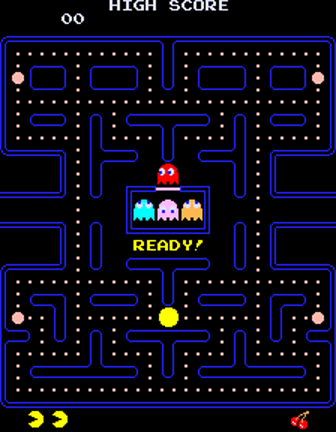
\includegraphics[scale=0.5]{pacman_level.png}
\caption{Pacman level screenshot: \cite{Pittman2011} }
\label{fig:Pacman}
\end{figure}


On figure \ref{fig:Pacman}, the setup for a level is displayed. The following elements in the game, within a single level, are the following:

\begin{itemize}
\item maze\\
The maze is the area of which the Pacman and ghosts navigates around throughout a level. There exists many different mazes which depends on the version of Pacman.
\item Pacman\\
Pacman is the playing agent that is navigated throughout the levels by moving up, down, left and right.
\item Ghosts\\
The ghosts, as seen on figure \ref{fig:Pacman}, is Blinky, Pinky, Inky and Clyde. They emerge from the center of the maze and chases the Pacman throughout the level, each using unique behaviours to catch him. Description of the ghost behaviours can be found in section XX.
\item dots and energizers\\
The dots within the maze functions as the foundation for winning a level in Pacman. Once all the dots are picked up/eaten by Pacman, the level is won.\\
The dots does however also grant points to the player.\\
Each dot is worth 10 points. In the original game, as stated by Pittman, 2011 \cite{Pittman2011}, there are 240 dots in total which amounts to 2400 points.

Energizers, which can be seen on figure \ref{fig:Pacman} as 4 bigger dots placed in each corner of the maze also grants points. 50 points each.
In combination, the total amount of points acquired by dots and energizers are  2600. The energizers does however also alter the state of the ghosts into a mode of which it is possible for the Pacman to eat the ghosts and thereby also acquiring points for a limited amount of time.\\
While the ghosts remain in the state of "fleeing" caused by the Pacman eating the energizer, each consecutive eaten ghost will result in twice as many points as the previus eaten ghost, whereof the first ghost gains the player 200 points.\\
If the player succesfully eats all four ghosts wile the "fleeing" state is active, the player acquire a total of 3000 points.\\

If all ghosts are consumed under the "fleeing" state of each energizer, in combination with the points from the gathered dots the combined score is 14600.
\item fruits
\end{itemize}




\subsection{Player performance}
a. Identify pacman parameters to measure player performance. (from 4.B) Associate also with  previous research(other AI implementations in Pacman. What did they use to  identify “performance”?


b. Define “good” and “bad” performance based upon 5a. (assume that we use only win/lose conditions unless prior research has based performance indications upon other game parameter results)

c. Performance results. We identify “some” performance. Therefore we configure the following “alternation of ghost behavior” in “this” way.

\subsection{Genetic Algorithm(s)}

\subsubsection{GA definitions. (what it is, and how it works}
\subsubsection{GA and Pacman(how the two can be combined.(methods)}
we must identify possible implementations of "pacman parameters" to control fitness score.
